\chapter{Introducción a la computación cuántica}

En este capítulo vamos a introducirnos en el mundo de la computación cuántica. No nos adentraremos en la teoría de la mecánica cuántica y usaremos nociones básicas de matemáticas, concretamente del álgebra lineal. Existen multitud de fuentes que ahondan en el conocimiento aportado por las matemáticas, la física y las ciencias de la computación para cimentar la teoría que vamos a desarrollar a continuación. Nos remitimos a ellas si existe el deseo de conocer más sobre esta rama de la ciencia o incluso a cualquiera de los TFG de los miembros de este grupo presentados para el grado de matemáticas.

Antes de empezar, vamos a hablar sobre una notación muy usada en mecánica cuántica y que emplearemos a menudo en este y los siguientes capítulos.

\section{Notación de Dirac}

La notación $\ket{\psi}$ denominada \textit{ket} pertenece a la notación de Dirac y representa al vector $\psi$ de cierto espacio vectorial complejo como columna, mientas que $\bra{\psi}$ representa al \textbf{conjugado} de $\psi$ como una fila. Por tanto, $\bra{\psi'}\ket\psi$ o $\braket{\psi'}{\psi}$ denota el \textbf{producto escalar complejo} dado por

\begin{equation}
\dotproduct\psi{\psi'}=\sum_{i=1}^{n}\psi_i\overline{\psi'_i}
\end{equation}

Denotamos $\ket\psi\bra\psi$ como el \textbf{producto exterior}. Por la definición anterior dadas para \textit{bra} y \textit{ket} se trata de una matriz de dimensiones $n\times n$ donde $n$ es la dimensión del espacio complejo donde habita $\psi$. Al tratarse de una matriz cuadrada, podemos identificarla como la matriz asociada de un isomorfismo lineal $\C^n\to\C^n$.

\section{Qubit}

El \textbf{qubit} o \textbf{cúbit} es el sistema de información más básico de la computación cuántica. Se trata de un vector unitario de del espacio vectorial $\C^2$ con una base ortonormal prefijada que denotamos por $\{\ket0,\ket1\}$. A menudo, a estos vectores ortonormales se les identifica con dos vectores de $\C^2$, habitualmente $\twovector{1}{0}$ y $\twovector{0}{1}$.

Esta elección de la base no se realiza de manera arbitraria, si no que los estados $\{\ket0,\ket1\}$ nos ayudarán a representar los valores de los bits clasicos 0 y 1. Pero, a diferencia de los bits, un qubit puede encontrarse en una \textbf{superposición} de los estados de la base, es decir, un qubit $\ket\psi$ se expresa como:
\begin{equation}
\ket{\psi}=\alpha\ket0+\beta\ket1,\mathrm{\ donde\ }\alpha,\beta\in\C.
\end{equation}

A los valores $\alpha$ y $\beta$ se les conoce como \textbf{amplitudes} del estado $\ket0$ y $\ket1$, respectivamente. Como un qubit es un vector unitario, los valores $\alpha$ y $\beta$ deben cumplir:
\begin{equation}
|\alpha|^2 + |\beta|^2 = 1
\end{equation}

Esto se conoce como la \textbf{restricción de normalización}.

Un concepto muy importante es el proceso de obtención de información que nos proporciona un qubit. Dicho proceso se conoce como \textbf{medir}.

\subsection{Medición de un qubit}

Pese a que un qubit se pueda encontrar en una superposición de estados de la base mencionada, la información que podemos extraer de este no es más que un valor de bit clásico. Esto se debe a que para obtener esta información hay que realizar los que se conoce como \textit{medida} sobre el qubit. Cuando se mide un qubit, este colapsa a uno de los dos estados de la base $\{\ket0,\ket1\}$, y por lo tanto, al igual que con los bits clásicos, solo hay dos posibles resultados.

Dado un qubit en el estado $\ket{\psi}=\alpha\ket0+\beta\ket1$, la probabilidad de obtener el estado $\ket0$ o $\ket1$ viene determinada por el cuadrado de las amplitudes de ambos. De esta forma, se tiene que $|\alpha|^2$ representa la probabilidad de obtener el estado $\ket0$, mientras que $|\beta|^2$ es la probabilidad de obtener el estado $\ket1$ al realizar una medición. Tras la medición, el estado actual es el obtenido por la medición.

Este proceso es irreversible, una vez realizada la medición, no se puede recuperar el estado original del qubit. Además, la elección de la base en la que medimos no es única. Una base alternativa relevante es $\{\ket+,\ket-\}$, donde $\ket+=\dfrac{1}{\sqrt{2}}(\ket0+\ket1)$ y $\ket-=\dfrac{1}{\sqrt{2}}(\ket0-\ket1)$. Se verifica que $\ket+$ y $\ket-$ son ortonormales entre sí.

Ejemplifiquemos todo esto suponiendo que tenemos el estado $\ket\psi=\ket+$ al que vamos a aplicar una medición. Si lo hacemos respecto de la base $\{\ket0,\ket1\}$ obtendremos con una probabilidad idéntica del 50\% $\ket0$ o $\ket1$. Sin embargo, si medimos respecto de la base $\{\ket+,\ket-\}$ obtendremos un 100\% de las veces el resultado $\ket+$. 

Llegados a este punto, uno puede preguntarse cuales son las ventajas de utilizar qubits frene a bits clásicos si la información que podemos obtener de ellos sique siendo binaria. Por ello, vamos a mostrar algunos ejemplos muy relevantes a lo largo de este capítulo que muestran el potencial de los qubits.

\subsection{Experimento: Distribución de Clave Cuántica}

Hemos hablado en el capítulo anterior del logro que supone el algoritmo de factorización de enteros de Shor. Esto podría poner en entredicho la seguridad de la computación clásica actual basada principalmente en el algoritmo de \textbf{RSA} que sustenta su confianza en la complejidad del problema de factorizar grandes números.

Surge así el interés por descubrir nuevos algoritmos criptográficos que, mediante el uso de la computación cuántica, resuelvan este problema. Vamos a hablar sobre el primer algoritmo de clave cuántica, \textbf{BB84}, cuyo esquema fue planteado por primera vez en 1984 por \textit{Bennett y Brassard} [\cite{bennett1987quantum}].

Supongamos que Alice y Bob quieren comunicarse de manera privada empleando para ello una clave secreta. Disponen para ello de un canal clásico bidireccional y de otro cuántico unidireccional que parte de Alice hacia Bob. El problema es que una tercera persona, Eve tiene acceso a ambos canales sin que ellos lo sepan (ver figura \ref{fig:fig21}). Además, Eve puede no sólo observar el canal cuántico, sino que también puede tomar las partículas que pasen por él, medirlas y reenviarlas a Bob.

% Diagrama Alice, Bob, Eve de distribución de clave cuántica
\begin{figure}[!htb]
\begin{center}
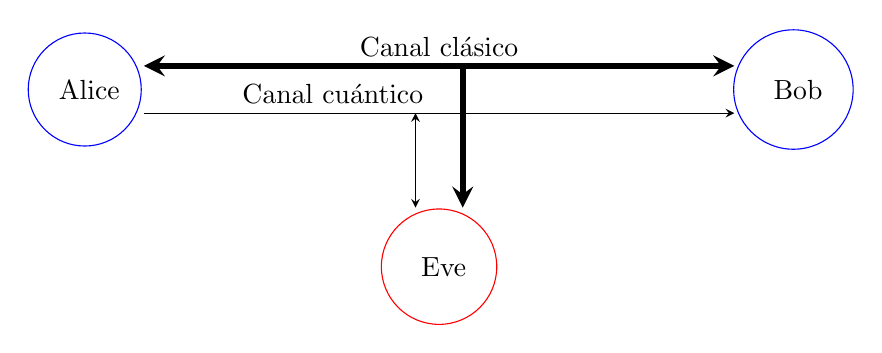
\begin{tikzpicture}[x=1.5cm, y=1.5cm]
    \node[circle,draw=blue] (v1) at (-3,0) {\ \ Alice\ \ };
    \node[circle,draw=blue] (v2) at (3,0) {\ \ \ Bob\ \ \ };
    \node[circle,draw=red] (v3) at (0,-1.5) {\ \ \ Eve\ \ \ };
    
    \draw[line width=0.8mm, {stealth}-{stealth}]  (-2.5,0.2) -- (2.5,0.2);
    \draw[line width=0.8mm, -{stealth}]  (0.2,0.2) -- (0.2,-1);
    
    \draw[-{stealth}]  (-2.5,-0.2) -- (2.5,-0.2);
    \draw[{stealth}-{stealth}]  (-0.2,-0.2) -- (-0.2,-1);
    
    \node at (0,0.2) [anchor=south] {Canal clásico};
    \node at (-0.9,-0.2) [anchor=south] {Canal cuántico};
\end{tikzpicture}
\end{center}
\caption{Esquema de distribución de clave cuántica.}
\label{fig:fig21}
\end{figure}

El primer paso del algoritmo es la elección de dos bases, como $\{\ket0,\ket1\}$ y $\{\ket+,\ket-\}$ y Alice procede a preparar una secuencia de bits. Para cada bit se elige aleatoriamente una de las bases para codificarlos, de manera que dicha codificación queda
\[\mathrm{bien\ }\begin{matrix}0\to\ket0\\1\to\ket1\end{matrix}\mathrm{,\ o\ bien\ }\begin{matrix}0\to\ket+\\1\to\ket-\end{matrix}\] 

en función de la base elegida. Tras la codificación, Alice envía a Bob la secuencia de qubits generada. Bob procede ahora a medir eligiendo, para cada qubit, una de las dos bases anteriormente citadas. Tras esta medición, tanto Alice como Bob hacen públicas las bases en las que la primera codificó y el segundo midió. Alrededor del 50\% de cada elección de estas bases coincidirá y los resultados asignados a estas elecciones se validan, mientras que el resto se desechan.

\begin{table}[htb]
\begin{tabular}{lll}
\rowcolor[HTML]{FFFFC7} 
Número del qubit & Base en la que codificó Alice & Base en la que midió Bob \\ 
\rowcolor[HTML]{FD6864} 
1                                & $\ket0,\ket1$                 & $\ket+,\ket-$            \\ 
\rowcolor[HTML]{9AFF99} 
2                                & $\ket0,\ket1$                 & $\ket0,\ket1$            \\ 
\rowcolor[HTML]{9AFF99} 
3                                & $\ket+,\ket-$                 & $\ket+,\ket-$            \\ 
\rowcolor[HTML]{FD6864} 
4                                & $\ket0,\ket1$                 & $\ket+,\ket-$            \\ 
\rowcolor[HTML]{9AFF99} 
5                                & $\ket+,\ket-$                 & $\ket+,\ket-$            \\ 
\rowcolor[HTML]{FD6864} 
6                                & $\ket+,\ket-$                 & $\ket0,\ket1$            \\ 
\rowcolor[HTML]{FD6864} 
7                                & $\ket+,\ket-$                 & $\ket0,\ket1$            \\ 
\rowcolor[HTML]{9AFF99} 
8                                & $\ket0,\ket1$                 & $\ket0,\ket1$            \\ 
\rowcolor[HTML]{9AFF99} 
9                                & $\ket0,\ket1$                 & $\ket0,\ket1$            \\ 
\rowcolor[HTML]{FD6864} 
10                               & $\ket0,\ket1$                 & $\ket+,\ket-$            \\ 
\rowcolor[HTML]{FFFFC7} 
...                              & ...                           & ...                      \\ 
\end{tabular}
\caption{Ejemplo de bases tomadas por Alice y Bob.}
\label{tab:tab21}
\end{table}

En el cuadro \ref{tab:tab21} se muestra un ejemplo de esta validación para los 10 primeros qubits de una secuencia. En verde aparecen los qubits para los que la base elegida por ambos coincidió y por tanto la medición de Bob arrojó el mismo resultado que la codificación de Alice. En rojo, por el contrario, aparecen aquellos cuyas bases no coincidieron y se descartan por no aportar información.

Ahora Alice y Bob pueden revelar una pequeña cantidad los valores obtenidos por cada uno, por ejemplo los $n$ primeros. Si todos esos valores coinciden, el canal es seguro y pueden utilizar el resto de los valores medidos no desvelados como clave. ¿Qué hubiera pasado si Eve hubiera intervenido el canal y hubiera tratado de medir los qubits antes de que lo hiciera Bob?

Al igual que Bob, Eve desconoce la base elegida por Alice para cada qubit, luego tendría que elegir una aleatoriamente  y realizar una medición. En el caso de escoger la misma que Alice (aunque Eve no podía tener la certeza hasta más tarde de haber acertado), no sólo podrá conocer el valor que codificó sino que además no está cambiando el estado del qubit y podrá reenviarlo a Bob inalterado. Esto ocurrirá en el 50\% de los casos; Sin embargo, en la otra mitad habrá elegido la base incorrecta modificando el estado del qubit y si Bob sí acierta con la base de Alice sólo tendrá un 50\% de posibilidades de medir el mismo valor que Alice codificó cuando debería serlo del 100\%.

Es así que Eve está introduciendo una variación en los estados en el 50\% de los qubits lo que supone que los valores de Alice y Bob diferirán en un 25\%. Si la cantidad de mediciones reveladas por ambos es de $n=20$ tras el intento de Eve de interceptar la comunicación, las probabilidades de no darse cuenta de la interferencia (no detectando ningún error) es de $0,75^{20}\approx0,32\%$. Tomando $n=30$ la probabilidad de pillar a Eve asciende a aproximadamente un 99,98\%, con lo que la certeza de garantizar la seguridad del canal es prácticamente absoluta con un tamaño de $n$ no necesariamente grande.

\section{Múltiples Qubits}

A lo largo de esta sección veremos cual es el comportamiento de un sistema cuántico cuando tenemos más de un qubit. Es aquí donde realmente podremos atisbar la capacidad de cómputo que tienen este tipo de máquinas.

En el física tradicional, si tenemos un sistema con $n$ partículas, cada una de ellas representada por un vector de dimensión 2, es el espacio vectorial que se genera es de dimensión $2n$. Esto se debe a que cada partícula se comporta de manera independiente y por tanto con ser capaces de modelizar el comportamiento individual de cada partícula tendremos representado todo el sistema. Es por ello que las dimensiones aumentan de manera lineal.

Sin embargo, esto no ocurre en mecánica cuántica. Las partículas ya no se comportan de manera independiente, si no que hay una dependencia entre ellos. Este efecto se llama \textit{entrelazamiento}, y entraremos en detalle posteriormente. 

Es por este motivo por el que no podemos modelizar los sistemas cuánticos con el comportamiento individual de cada partícula, si no que necesitaremos de una herramienta más potente, el \textbf{productor tensorial}.

\subsection{Producto Tensorial}

Supongamos que tenemos dos espacios vectoriales $\mathcal{V},\mathcal{W}$ de dimensiones $n$ y $m$ respectivamente. Entonces $\mathcal{V}\otimes\mathcal{W}$ es un espacio vectorial de dimension $n\times m$ y representa el producto tensorial de ambos espacios.

Además, supongamos que tenemos bases ortogonales para $\mathcal{V}$ y $\mathcal{W}$ dadas por:
\begin{equation}
\begin{split}
\mathcal{B}_v =\{\ket{v_i} |\ 1 \leq i \leq n \} \\
\mathcal{B}_w =\{\ket{w_j} |\ 1 \leq j \leq m \}
\end{split}
\end{equation}

Entonces una base $\mathcal{B}$ del espacio vectorial $\mathcal{V}\otimes\mathcal{W}$ se obtiene mediante el producto tensorial de los vectores de $\mathcal{B}_v$  y $\mathcal{B}_v$, es decir:
\begin{equation}
\mathcal{B} = \{\ket{v_i}\otimes\ket{w_j}|\ 1 \leq i \leq n,\ 1 \leq j \leq m \}
\end{equation}

Normalmente se aligera la notación y denotaremos $\ket{\phi}\otimes\ket{\psi}$ simplemente por $\ket{\phi}\ket{\psi}$ o incluso por $\ket{\phi\psi}$.

Por definición, el producto tensorial cumple las siguientes tres propiedades [\cite{nielsen2001quantum}]:
\begin{enumerate}
\item Dado un escalar z y un vector $\ket{v}$ de $\mathcal{V}$ y $\ket{w}$ de $\mathcal{W}$,\\
\begin{equation}
z(\ket{v}\otimes\ket{w})= (z\ket{v})\otimes\ket{w} = \ket{v}\otimes (z\ket{w})
\end{equation}

\item Para los vectores $\ket{v_1}$  y $\ket{v_2}$ de $\mathcal{V}$ y $\ket{w}$ de $\mathcal{W}$,\\
\begin{equation}
(\ket{v_1}+\ket{v_2})\otimes\ket{w}=\ket{v_1}\otimes\ket{w}+\ket{v_2}\otimes\ket{w}
\end{equation}

\item Para los vectores $\ket{v}$ de $\mathcal{V}$ y $\ket{w_1}$, $\ket{w_2}$ de $\mathcal{W}$,\\
\begin{equation}
\ket{v}\otimes (\ket{w_1}+\ket{w_2}) = \ket{v}\otimes\ket{w_1} +\ket{v}\otimes\ket{w_2} 
\end{equation}
\end{enumerate}

Por tanto, supongamos que tenemos dos qubits, cuyos espacios vectoriales están representados respectivamente por la base ortonormal estándar $\{\ket0,\ket1\}$. Entonces, el nuevo espacio vectorial 
generado por ambos qubits tiene como base los vectores $\{\ket{00},\ket{01},\ket{10},\ket{11}\}$, es decir, un espacio de dimensión 4. Sin embargo, este ejemplo no es demasiado ilustrativo(pues $2^n = 2n$ si $n=4$).

Así que supongamos que añadimos un tercer qubit a nuestro sistema de dos qubits. Entonces el nuevo espacio vectorial tendrá dimensión 8 ($2^3$) y su base viene dada por los vectores $\{\ket{000},\ket{001},\ket{010},\ket{011},\ket{100},\ket{101},\ket{110},\ket{111}\}$

Si repetimos estos cálculos pero utilizando la representación de la base como matri